  \documentclass[10pt, aspectratio=169]{beamer}

% --- CẤU HÌNH CƠ BẢN ---
\usepackage[utf8]{inputenc}
\usepackage[T1]{fontenc}
\usepackage[vietnamese]{babel} % Hỗ trợ tiếng Việt

% --- THEME VÀ MÀU SẮC ---
\usetheme{Madrid} 
\usecolortheme{dolphin} 
\setbeamertemplate{navigation symbols}{} % Tắt thanh điều hướng
\setbeamertemplate{headline}{} % Tắt headline

% --- CÁC GÓI PHỤ TRỢ ---
\usepackage{amsmath}
\usepackage{amsfonts}
\usepackage{graphicx}
\usepackage{booktabs} 
\usepackage{tikz}

% --- THÔNG TIN BÀI THUYẾT TRÌNH ---
\title[Learnability of Algorithms in NNs]{Nghiên cứu về khả năng học chính xác thuật toán\\
của mạng nơ-ron}

\subtitle{Báo cáo tiến độ giữa kỳ\\[0.4em]
    \footnotesize Bài báo: \textit{Learning to Add, Multiply, and Execute Algorithmic Instructions Exactly with Neural Networks}
}

\author[Nhóm 11]{\textbf{Nhóm 11}\\[0.6em]
    \small
    23127006 -- Trần Nguyễn Khải Luân\\
    23127179 -- Nguyễn Bảo Duy\\
    23127333 -- Trương Quốc Cường\\
    23127539 -- Nguyễn Thanh Tiến
}

\institute[HCMUS]{%
    Trường Đại học Khoa học Tự nhiên, ĐHQG-HCM\\[0.4em]
    \textit{Giảng viên hướng dẫn:} Lê Nhựt Nam
}

\date{\today}




\begin{document}

% --- SLIDE TIÊU ĐỀ ---
\begin{frame}
    \titlepage
\end{frame}

% --- SLIDE MỤC LỤC ---
\begin{frame}{Nội dung trình bày}
    \tableofcontents
\end{frame}

% =============================================================================
% PHẦN 1: GIỚI THIỆU
% =============================================================================
\section{1. Giới thiệu}

% --- TRANSITION SLIDE PHẦN 1 ---
\begin{frame}
    \centering
    \Huge \textbf{Phần 1: Giới thiệu}
\end{frame}

% 1.1
\begin{frame}{1.1. Bức tranh hiện tại: Học sâu trên miền liên tục}

  \begin{block}{Nhận dạng mẫu (Pattern Recognition)}
    Học sâu đã rất thành công trong:
    \begin{itemize}
      \item \textbf{Thị giác máy tính:} 
            Phân loại ảnh, nhận diện vật thể.
      \item \textbf{Xử lý ngôn ngữ tự nhiên:} 
            Dịch máy, phân tích cảm xúc.
    \end{itemize}
  \end{block}

  \vspace{0.4em}
  \textbf{Lý do thành công (trên miền liên tục):}
  \begin{itemize}
    \item Dữ liệu là tín hiệu \textbf{liên tục, trơn} (continuous, smooth).
    \item Mục tiêu: \textbf{xấp xỉ hàm liên tục} từ dữ liệu mẫu
          bằng thuật toán Gradient Descent.
  \end{itemize}

\end{frame}

% 1.1 - Frame 2 (tiếp)
\begin{frame}{1.2. Bức tranh hiện tại: Khoảng trống suy luận (Reasoning)}

    \begin{block}{Nhu cầu của trí tuệ nhân tạo thế hệ mới}
        Các ứng dụng hiện đại (Lập trình, Toán học) đòi hỏi \textbf{suy luận} – 
        thực thi quy tắc thuật toán, không chỉ nhận dạng mẫu.
    \end{block}
    
    \textbf{Hạn chế của mô hình ngôn ngữ lớn hiện tại:}
    \begin{itemize}
        \item Sai các phép toán đơn giản với số lớn.
        \item Lập luận logic không nhất quán.
        \item Không duy trì được quy tắc trên chuỗi dài (vòng lặp, đệ quy).
    \end{itemize}
    $\to$ \textit{Mạng chủ yếu học “dự đoán xác suất” chứ không nắm chắc “quy tắc logic”.}

    \vspace{0.8em}

    Hiện nay, RNN và Transformer đã được chứng minh là \textbf{có khả năng biểu diễn
    (expressibility)} mọi loại lệnh và thuật toán phức tạp.  
    Tuy nhiên, việc \textbf{Gradient Descent có khả năng học (learnability) đúng bộ trọng số đó hay không}
    lại là một câu chuyện hoàn toàn khác.  

    \vspace{0.3em}

    Đây chính là \textbf{khoảng trống nghiên cứu} đặt nền tảng cho bài báo.
    
\end{frame}

% 1.1 - Frame 3 (tiếp)
% \begin{frame}{1.1. Bức tranh hiện tại: Từ khả năng biểu diễn đến khả năng học}

%     \begin{columns}
%         % Cột 1
%         \column{0.48\textwidth}
%         \begin{block}{Khả năng biểu diễn (Expressibility)}
%             \begin{minipage}[t][3.2cm][t]{\linewidth} 
%                 \textit{Mạng nơ-ron \textbf{có thể} thực thi thuật toán không?}
%                 \begin{itemize}
%                     \item \textbf{Câu trả lời:} Có.
%                     \item RNN, Transformer: có khả năng tính toán tương đương máy Turing.
%                     \item Tồn tại bộ tham số thực thi đúng thuật toán.
%                 \end{itemize}
%             \end{minipage}
%         \end{block}
        
%         % Cột 2
%         \column{0.48\textwidth}
%         \begin{block}{Khả năng học (Learnability)}
%             \begin{minipage}[t][3.2cm][t]{\linewidth}
%                 \textit{Thuật toán hạ dốc (Gradient Descent) có \textbf{học được} thuật toán đó không?}
%                 \begin{itemize}
%                     \item \textbf{Câu trả lời:} Chưa rõ.
%                     \item Expressibility $\neq$ Learnability.
%                     \item Thực nghiệm: thường chỉ đạt nghiệm xấp xỉ.
%                 \end{itemize}
%             \end{minipage}
%         \end{block}
%     \end{columns}

% \end{frame}


% 1.4
\begin{frame}{1.3. Mục tiêu bài toán}

    \textbf{Câu hỏi chính:}
    \begin{quote}
        Mạng nơ-ron, khi huấn luyện bằng Gradient Descent trong chế độ NTK,
        có thể học \textbf{đúng hoàn toàn} các thuật toán rời rạc
        (cộng, nhân, \ldots) hay không?
    \end{quote}
    \vspace{0.8em}
    \textbf{Trọng tâm:}
    \begin{itemize}
        \item Không bàn về “có biểu diễn được hay không”.
        \item Chỉ hỏi: “có \textbf{học ra đúng} thuật toán hay không”.
        \item Hướng tới trí tuệ nhân tạo (AI) thực sự \textbf{thực thi quy tắc}, không chỉ bắt chước dữ liệu.
    \end{itemize}

\end{frame}


\begin{frame}{1.4. Ý nghĩa khoa học}

\begin{enumerate}

    \item \textbf{Làm rõ khả năng của Gradient Descent trong việc học hàm rời rạc}
    \begin{itemize}
        \item Chỉ ra rằng dù tối ưu diễn ra trong miền liên tục, GD vẫn có thể học chính xác các quy tắc rời rạc (bitwise functions) khi được biểu diễn bằng template.
        \item Phân tích động lực học của GD bằng NTK, chứng minh điều kiện để dự đoán hội tụ về đáp án rời rạc.
    \end{itemize}

    \item \textbf{Chuyển trọng tâm từ “biểu diễn được” sang “học được”}
    \begin{itemize}
        \item Các kết quả Turing-complete trước đây chỉ nói về \textit{expressivity};
        bài báo này chứng minh \textit{learnability}, mạng thật sự học được thuật toán từ dữ liệu.
    \end{itemize}

    \item \textbf{Nhắm tới tính đúng tuyệt đối (exact execution)}
    \begin{itemize}
        \item Mục tiêu không chỉ là xấp xỉ hay đúng với xác suất cao.
        \item Chứng minh một mạng hai lớp có thể thực thi thuật toán \textbf{chính xác 100\%} khi lặp block đã học.
    \end{itemize}

\end{enumerate}

\end{frame}



% 1.6
\begin{frame}{1.5. Ý nghĩa thực tiễn}

\begin{itemize}
    \item \textbf{Đặt nền móng cho các mô hình AI có thể học thuật toán đáng tin cậy}  
    Cung cấp khung lý thuyết cho việc để mạng nơ-ron học chính xác các bước thuật toán, thay vì chỉ bắt chước mẫu dữ liệu.

    \item \textbf{Hỗ trợ phát triển hệ thống AI yêu cầu độ chính xác cao}  
    Các lĩnh vực như kiểm chứng, mật mã, phân tích chương trình, hay hệ thống an toàn có thể hưởng lợi từ khả năng học quy tắc chính xác ở mức bit.

    \item \textbf{Gợi ý hướng xây dựng mô hình giải toán / lập luận mạnh hơn}  
    Bằng cách hiểu điều kiện để mạng học được quy trình rời rạc, nghiên cứu tương lai có thể thiết kế mô hình tổng quát hoá tốt hơn cho reasoning.

\end{itemize}

\end{frame}




% =============================================================================
% PHẦN 2: KIẾN THỨC CƠ SỞ
% =============================================================================
\section{2. Kiến thức cơ sở}

% --- TRANSITION SLIDE PHẦN 2 ---
\begin{frame}
    \centering
    \Huge \textbf{Phần 2: Kiến thức cơ sở}
\end{frame}

% 2.1
\begin{frame}{2.1. Mâu thuẫn: Miền liên tục vs. Miền rời rạc}

    \begin{block}{Ý tưởng cốt lõi}
        Miền liên tục và miền rời rạc khác nhau ở \textbf{mức độ nhạy cảm với sai số}.
    \end{block}

    \vspace{1em}

    \textbf{Trong bài toán liên tục:}  
    Sai số nhỏ thường không gây vấn đề lớn. Ví dụ: $0.99 \approx 1.00$

    \vspace{0.5em}

    \textbf{Trong bài toán rời rạc:}  
    Chỉ cần sai \textbf{một bit nhớ} là toàn bộ kết quả hỏng hoàn toàn — không còn khái niệm “gần đúng”. Ví dụ:

\[
\begin{array}{ccccccc}
    & 1 & 1 & 1 & 1 & 1 & 1 \\
    + & 0 & 0 & 0 & 0 & 0 & 1 \\
    \hline
    1 & 0 & 0 & 0 & 0 & 0 & 0 \\
\end{array}
\]

    \vspace{0.2em}

    \begin{block}{Hệ quả}
        Gradient Descent — vốn dựa trên \textbf{tính trơn (smoothness)} — gặp khó khăn khi phải học các hàm rời rạc có độ nhạy cao với sai số.
    \end{block}

\end{frame}

% 2.2
\begin{frame}{2.2. Công cụ phân tích: Neural Tangent Kernel (NTK)}

\begin{block}{Neural Tangent Kernel (NTK)}
    \begin{itemize}
        \item NTK mô tả hành vi học của mạng neural khi \textbf{chiều rộng tiến đến vô hạn}.
        \item Trong miền (regime) này, mạng hành xử như một \textbf{mô hình tuyến tính} trong một không gian đặc trưng cố định.
        \item NTK cho phép \textit{phân tích chính xác}: mạng sẽ học ra hàm gì sau khi train.
    \end{itemize}
\end{block}

\vspace{0.7em}

\begin{block}{Ý nghĩa đối với bài báo}
    Bài báo dùng NTK để \textit{chứng minh lý thuyết learnability}, nên NTK đóng vai trò là công cụ toán học để mô hình hoá chính xác quá trình học của mạng.
\end{block}

\end{frame}

% 2.3
\begin{frame}{2.3. Đặc điểm thuật toán số học}

Các thuật toán số học cổ điển (cộng, nhân nhị phân) có những tính chất nổi bật:

\begin{itemize}

    \item \textbf{Cục bộ (Local):}  
    Mỗi bước chỉ thao tác lên một phần rất nhỏ của trạng thái  
    (ví dụ: một cặp bit và bit nhớ).  
    Điều này cho phép mô tả thuật toán dưới dạng các \textit{quy tắc local}.

    \item \textbf{Lặp lại (Iterative):}  
    Cùng một quy tắc được áp dụng lặp đi lặp lại cho từng vị trí bit.  
    Đây là dạng tính toán “template” - một bước mẫu được nhân bản theo chiều dài chuỗi.

    \item \textbf{Độc lập theo vị trí (Position-wise independence):}  
    Quy tắc xử lý tại vị trí $i$ không phụ thuộc vào giá trị tại các vị trí xa,  
    mà chỉ phụ thuộc vào trạng thái rất gần (bit bên cạnh hoặc carry).
    Điều này giúp tách thuật toán thành các bước nhỏ có thể học độc lập.

\end{itemize}

\vspace{0.3cm}
\centering
$\Rightarrow$ \textbf{Bài báo khai thác chính 3 đặc tính này để xây dựng \textit{local templates},}
\\
\textit{giúp mạng nơ-ron học từng bước của thuật toán một cách rõ ràng và hiệu quả.}

\end{frame}


% 2.4
\begin{frame}{2.4. Tính đầy đủ Turing (Turing-completeness)}

\begin{block}{Định nghĩa}
Một hệ thống được gọi là \textbf{Turing-complete} nếu nó có khả năng mô phỏng
\textbf{mọi thuật toán khả tính}, tương đương sức mạnh của một máy Turing.
\end{block}

\vspace{1em}

Để đạt tính đầy đủ Turing, một tập lệnh hoặc mô hình tính toán cần thỏa mãn ba
năng lực cốt lõi:

\begin{enumerate}
    \item \textbf{Thao tác bộ nhớ (Memory Manipulation)}
    \begin{itemize}
        \item Có khả năng đọc, ghi và cập nhật trạng thái bộ nhớ.
        \item \textit{Ví dụ:} Gán giá trị, tăng/giảm biến: $x = x + 1$.
    \end{itemize}

    \item \textbf{Logic điều kiện (Conditional Logic)}
    \begin{itemize}
        \item Cho phép ra quyết định dựa trên trạng thái hiện thời.
        \item \textit{Ví dụ:} Kiểm tra dấu hoặc so sánh: nếu $x < 0$ thì nhảy đến nhãn A.
    \end{itemize}

    \item \textbf{Điều khiển luồng (Control Flow / Looping)}
    \begin{itemize}
        \item Hỗ trợ lặp hoặc nhảy có điều kiện, cho phép chạy chương trình với độ dài tùy ý.
        \item \textit{Ý nghĩa:} Cơ chế LOOP/GOTO giúp mở rộng tính toán trên dữ liệu không giới hạn.
    \end{itemize}
\end{enumerate}



\end{frame}


\begin{frame}{Ví dụ về Turing-complete}
    \begin{block}{Lệnh \texttt{Substract and Branch if Negative (SBN)}}
        \texttt{SBN x, y, L} thực hiện:
        \[
        x = x - y; \quad \text{nếu } x < 0 \text{ thì nhảy đến } L.
        \]

        Dù chỉ có 1 loại lệnh duy nhất, nó vẫn đủ 3 thành phần:
        \begin{itemize}
            \item Trừ $\Rightarrow$ cập nhật trạng thái
            \item Kiểm tra âm $\Rightarrow$ điều kiện
            \item Nhảy $\Rightarrow$ điều khiển luồng
        \end{itemize}

        \textbf{$\Rightarrow$ SBN một mình đã Turing-complete.}
    \end{block}
\end{frame}

% =============================================================================
% PHẦN 3: PHÁT BIỂU BÀI TOÁN
% =============================================================================
\section{3. Phát biểu bài toán}

% --- TRANSITION SLIDE PHẦN 3 ---
\begin{frame}
    \centering
    \Huge \textbf{Phần 3: Phát biểu bài toán}
\end{frame}

% 3.1
\begin{frame}{3.1. Mục tiêu tổng quát}
    \textbf{Mục tiêu của bài toán:}

    \begin{block}{Câu hỏi trung tâm}
        Liệu một mạng nơ-ron kết nối đầy đủ hai tầng, được huấn luyện bằng 
        \textbf{gradient descent trong chế độ NTK}, có thể học và thực thi 
        \textbf{chính xác tuyệt đối} các thuật toán rời rạc ở cấp độ bit hay không?
    \end{block}


    Các thuật toán được xét:
    \begin{itemize}
    \item \textbf{Hoán vị nhị phân} — chuyển vị trí các bit theo quy tắc cố định.
    \item \textbf{Cộng nhị phân} — cộng hai số có lan truyền bit nhớ (carry).
    \item \textbf{Nhân nhị phân} — lặp lồng nhau theo từng bit (nested loops).
    \item \textbf{Lệnh SBN} — một lệnh Turing-complete, mô phỏng mọi thuật toán qua lặp lại.
\end{itemize}


\end{frame}

% % 3.2
% \begin{frame}{3.2. Bộ thuật toán được xét}
%     \textbf{1. Binary Permutation}
%     \begin{itemize}
%         \item Đại diện cho routing/indexing
%         \item Chuyển bit từ vị trí này sang vị trí khác
%     \end{itemize}

%     \textbf{2. Binary Addition}
%     \begin{itemize}
%         \item Thuật toán cộng logic có carry
%     \end{itemize}

%     \textbf{3. Binary Multiplication}
%     \begin{itemize}
%         \item Thuật toán nhiều vòng lặp (nested iteration)
%     \end{itemize}

%     \textbf{4. SBN (Subtract-and-Branch-if-Negative)}
%     \begin{itemize}
%         \item Một lệnh duy nhất nhưng \textbf{Turing-complete}
%         \item Mọi thuật toán đều mô phỏng bằng việc lặp SBN nhiều lần
%     \end{itemize}
% \end{frame}

\begin{frame}{3.2. Phương hướng chứng minh}

    \begin{enumerate}
        \item \textbf{Thuật toán được phân rã thành các template cục bộ}\\
        Chuẩn hoá thuật toán thành các bước xử lý cục bộ trên trạng thái nhị phân
        (template $X \rightarrow Y$).

        \item \textbf{Tập dữ liệu huấn luyện trực giao}\\
        Xây dựng tập dữ liệu huấn luyện được mã hoá trực giao theo từng block,
        bảo đảm mỗi template được học độc lập (tính học được cục bộ).

        \item \textbf{Phân tích NTK}\\
        Sử dụng NTK để chứng minh gradient descent trên mạng hai tầng
        học đúng ánh xạ của từng template với khoảng cách an toàn (margin) $> 0$.

        \item \textbf{Thực thi bằng vòng lặp}\\
        Lặp lại các block / template để thực thi các thuật toán dài
        (nhiều bước, nhiều vị trí bit).

        \item \textbf{Mở rộng tới tính đầy đủ Turing (SBN)}\\
        Chứng minh các template SBN học được mà SBN turing-complete
        $\Rightarrow$ khung đề xuất đủ năng lực học mọi hàm có thể tính được.
    \end{enumerate}

\end{frame}

\begin{frame}{Ví dụ minh họa}

\begin{center}
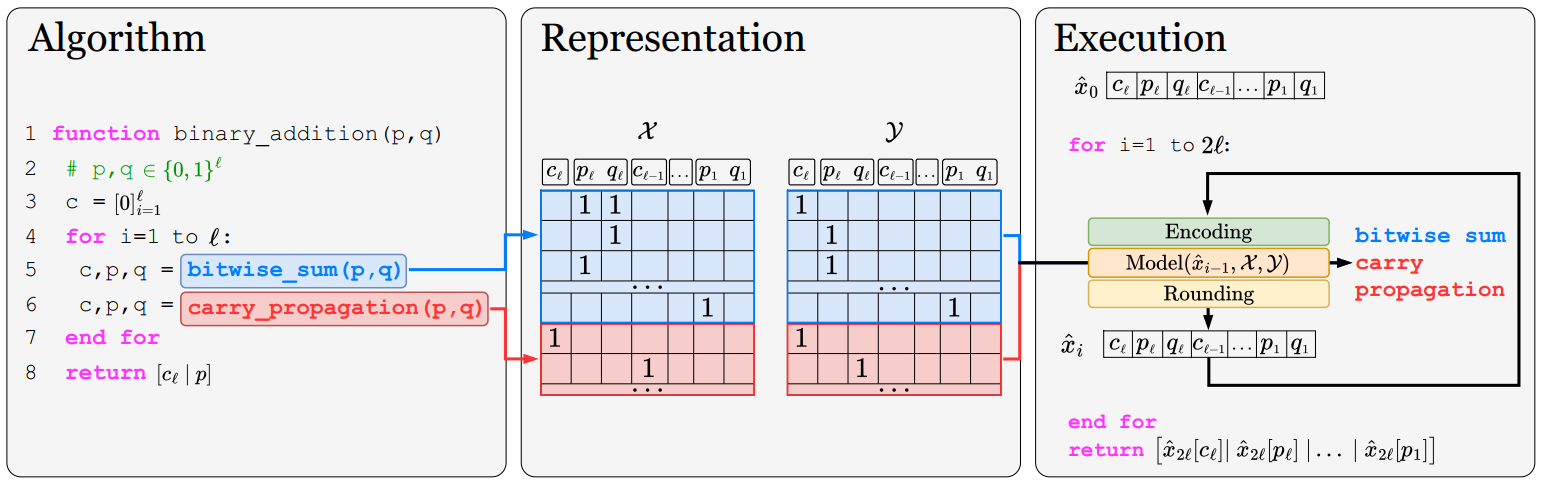
\includegraphics[width=0.8\textwidth]{vd.png}
\end{center}

\begin{itemize}

    \item \textbf{Algorithm (trái):}
    Thuật toán cộng được tách thành hai bước mẫu (template):
    \emph{bitwise\_sum} và \emph{carry\_propagation}.

    \item \textbf{Representation (giữa):}
    Mỗi bước mẫu được mã hóa thành cặp \((X \rightarrow Y)\), 
    trong đó:
    \(X\) là trạng thái đầu vào (p, q, carry),  
    \(Y\) là đầu ra đúng của bước đó.

    \item \textbf{Execution (phải):}
    Ở bước \(i\), mô hình nhận \(\hat{x}_{i-1}\), dự đoán đầu ra,
    làm tròn để thu được \(\hat{x}_{i}\), và lặp lại để hoàn thành thuật toán.

\end{itemize}


\vspace{0.1cm}

% \begin{block}{Điểm quan trọng}
% Mô hình chỉ \textbf{học} ở phần Representation (các cặp \((X,Y)\)).
% Khi chạy thuật toán (Execution), mô hình \textbf{không học thêm} mà chỉ áp dụng
% các template đã học.
% \end{block}

\end{frame}

% 3.3
\begin{frame}{3.3. Đặc tả hình thức: Đầu vào (Input)}
    Đầu vào là \textbf{trạng thái thuật toán} tại một bước thực thi bất kỳ:
    \begin{itemize}
        \item Các bit của toán hạng thứ nhất
        \item Các bit của toán hạng thứ hai
        \item Bit nhớ
        \item Chỉ số vị trí đang xét (index/step)
        \item Các bit trạng thái phụ thuộc thuật toán
    \end{itemize}

    \vspace{0.5em}

    Ký hiệu:
    \[
        \mathbf{x} \in \{0,1\}^d
    \]
    với $d$ là tổng số bit mã hóa trạng thái.
\end{frame}

% 3.3
\begin{frame}{3.4. Đặc tả hình thức: Đầu ra (Output)}
    Đầu ra là vector nhị phân biểu diễn:
    \begin{itemize}
        \item Bit kết quả tại vị trí hiện tại
        \item Trạng thái mới (bit nhớ)
        \item Tín hiệu lặp cho bước tiếp theo
    \end{itemize}

    \vspace{0.5em}
    Ký hiệu hình thức: \\[0.3em]
    \[
        \mathbf{y} \in \{0,1\}^k
    \]

    \vspace{0.5em}
    Mỗi bước: đầu ra được làm tròn để cập nhật trạng thái:
    \[
        \mathbf{x}_{t+1} = \text{round}(f_\theta(\mathbf{x}_t))
    \]
\end{frame}

% % 3.5
% \begin{frame}{3.5. Mô hình học: 2-layer MLP trong NTK regime}
%     Ta xét mạng nơ-ron fully-connected 2 tầng:
%     \[
%         f_\theta : \{0,1\}^d \to \mathbb{R}^k
%     \]

%     Được huấn luyện bằng gradient descent trên tập dữ liệu:
%     \[
%         (\mathbf{x}_i, \mathbf{y}_i), \quad \mathbf{y}_i = \text{instruction}(\mathbf{x}_i)
%     \]

%     Trong \textbf{NTK regime}:
%     \begin{itemize}
%         \item Mạng hội tụ về \textit{NTK mean predictor}
%         \item Giúp phân tích lý thuyết động lực học của quá trình học
%         \item Là nền tảng để chứng minh learnability
%     \end{itemize}
% \end{frame}

% % 3.6
% \begin{frame}{3.6. Mô hình thuật toán (Algorithm Model)}
%     Mỗi thuật toán rời rạc được mô tả như một \textbf{quy tắc cục bộ}:
%     \[
%         \mathbf{y} = g(\mathbf{x})
%     \]

%     Với đặc tính:
%     \begin{itemize}
%         \item $g$ là ánh xạ đúng của thuật toán (bit-level)
%         \item Với addition: sinh bit tổng + carry mới
%         \item Với multiplication: tính partial products + propagate carries
%         \item Với SBN: cập nhật bộ đếm lệnh (program counter)
%     \end{itemize}

%     Thuật toán hoạt động lặp:
%     \[
%         \mathbf{x}_{t+1} = g(\mathbf{x}_t)
%     \]
% \end{frame}

% % 3.7
% \begin{frame}{3.7. Bài toán học chính xác (Exact Learnability Problem)}
%     \textbf{Câu hỏi chính:}

%     \begin{block}{Exact Learnability}
%         Tồn tại điều kiện nào (kiến trúc, dữ liệu, template, kích thước block)
%         để mạng 2 tầng trong NTK regime học được ánh xạ $g$ \textbf{một cách CHÍNH XÁC}?
%     \end{block}

%     Yêu cầu:
%     \[
%         \forall \mathbf{x} \in \text{Domain}, 
%         \quad \text{round}(f_\theta(\mathbf{x})) = g(\mathbf{x})
%     \]

%     Và thuật toán được tái tạo đúng:
%     \[
%         \mathbf{x}_{t+1} = \text{round}(f_\theta(\mathbf{x}_t))
%     \]

%     \textbf{→ Mạng phải sinh đúng toàn bộ thuật toán khi lặp lại nhiều bước.}
% \end{frame}

% =============================================================================
% PHẦN 4: CÔNG TRÌNH LIÊN QUAN
% =============================================================================
\section{4. Công trình liên quan}

% --- TRANSITION SLIDE PHẦN 4 ---
\begin{frame}
    \centering
    \Huge \textbf{Phần 4: Công trình liên quan}
\end{frame}

% Slide chứa bảng so sánh (Update theo hình ảnh)
\begin{frame}{4.1. Các công trình liên quan}
    \begin{table}
        \centering
        \renewcommand{\arraystretch}{1.5} % Giãn dòng cho dễ đọc
        \resizebox{\textwidth}{!}{%
            \begin{tabular}{|p{0.20\linewidth}|p{0.26\linewidth}|p{0.26\linewidth}|p{0.26\linewidth}|}
                \hline
                \textbf{Hướng tiếp cận} & \textbf{Phương pháp (ngắn gọn)} & \textbf{Ưu điểm} & \textbf{Nhược điểm} \\
                \hline

                % --- Row 1 ---
                 Siegelmann \& Sontag (1995) -- RNN Turing-complete &
                Chứng minh RNN có thể mô phỏng mọi thuật toán &
                Sức mạnh biểu đạt rất lớn $\Rightarrow$ RNN có khả năng biểu đạt mọi quy tắc thuật toán. &
                Không đề cập đến khả năng học bằng gradient descent \\
                \hline

                % --- Row 2 ---
                Kaiser \& Sutskever (2016) -- Neural GPU &
                Thiết kế Neural GPU để học cộng \& nhân nhị phân bằng cập nhật song song. &
                Học được cộng/nhân với khả năng tổng quát hoá trên chuỗi dài. &
                Kết quả mang tính thực nghiệm; không có bảo đảm lý thuyết về học chính xác. \\
                \hline

                % --- Row 3 ---
                Pérez et al. (2021) -- Transformer Turing-complete &
                Chứng minh Transformer có thể mô phỏng máy Turing khi cấu hình đúng. &
                Cho thấy Transformer cũng có khả năng biểu diễn thuật toán mạnh. &
               Không phân tích học bằng gradient; không đảm bảo học chính xác thuật toán ở mức bit.\\
                \hline

            \end{tabular}%
        }
    \end{table}
\end{frame}

\begin{frame}{4.2. Đóng góp chính của công trình}

Công trình này đưa ra một kết quả mới và quan trọng:

\vspace{0.2cm}

\begin{block}{Điểm đột phá}
Lần đầu tiên chứng minh được rằng một mạng nơ-ron hai tầng,
khi được huấn luyện bằng gradient descent,
có thể học \emph{chính xác} từng bước của một thuật toán rời rạc.
Kết quả đạt được nhờ cách biểu diễn bằng template và phân tích trong khuôn khổ NTK.
\end{block}

\vspace{0.2cm}

Điểm này giúp giải quyết một hạn chế chung của các hướng nghiên cứu trước đó:
mặc dù mô hình có thể biểu diễn thuật toán,  
nhưng \emph{không có bảo đảm} rằng quá trình học sẽ tìm ra đúng thuật toán.

\vspace{0.3cm}

Kết quả của bài báo thu hẹp khoảng cách giữa:
\begin{itemize}
    \item \textbf{Expressivity}: khả năng mạng nơ-ron biểu diễn thuật toán, và
    \item \textbf{Learnability}: khả năng học được thuật toán thông qua Gradient Descent.
\end{itemize}

\end{frame}

% --- SLIDE KẾT THÚC ---
\begin{frame}
    \centering
    \Huge \textbf{Cảm ơn Thầy và các bạn đã lắng nghe!}
\end{frame}

\end{document}